\chapter{Specifikacija programske potpore}

\section{Funkcionalni zahtjevi}

\noindent \textbf{Dionici:}

\begin{packed_enum}

	\item Korisnici
	\begin{enumerate}
		\item Registrirani/prijavljeni
		\item Neregistrirani
	\end{enumerate}
	\item Moderator
	\item Razvojni tim

\end{packed_enum}



\noindent \textbf{Aktori i njihovi funkcionalni zahtjevi:}


\begin{packed_enum}
	\item  \underbar{Neregistrirani/neprijavljeni korisnik (inicijator) može:}

	\begin{packed_enum}

		\item Pregledati sve recepte
		\item Sortirati i filtrirati recepte po raznim argumentima
		\item Filtrirati recepte po sastojcima
		\item Pretražiti recepte po imenu/autoru
		\item Registrirati se

	\end{packed_enum}

	\item  \underbar{Registrirani/prijavljeni korisnik (inicijator) može:}

	\begin{packed_enum}

		\item Raditi sve kao i neregistrirani/neprijavljeni korisnik
		\item Dodati vlastiti recept (Dodani recept mora sadržavati maksimalno 5 slika, te po jedan sastojak i korak pripreme)
		\item Urediti vlastiti recept (obrisati/dodati sastojke, urediti i dodati korake i opis)
		\item Dodavati komentare na recepte
		\item Brisati vlastite komentare\newline \newline \newline
	\end{packed_enum}

	\item  \underbar{Moderator (inicijator) ima mogućnost:}

	\begin{packed_enum}

		\item Brisanja i dodavanja komentara, ali ne i ocjenjivanja recepata
		\item Brisanja recepata
		\item Brisanja korisničkih računa
		\item Pregleda svih korisnika
	\end{packed_enum}

	\item  \underbar{Baza podataka (sudionik) mora moći:}

	\begin{packed_enum}

		\item Spremati sve podatke o receptima
		\item Spremati sve podatke o korisnicima
		\item Spremati sve podatke o moderatorima
		\item Izvršiti zadani upit i vratiti rezultat
	\end{packed_enum}
\end{packed_enum}


\eject



\subsection{Obrasci uporabe}

\subsubsection{Opis obrazaca uporabe}

\noindent \underbar{\textbf{UC1 - Sortiranje recepata po popularnosti}}
\begin{packed_item}

	\item \textbf{Glavni sudionik: } Korisnik
	\item  \textbf{Cilj:} Filtrirati recepte po popularnosti
	\item  \textbf{Sudionici:} Baza podataka
	\item  \textbf{Preduvjet:} -
	\item  \textbf{Opis osnovnog tijeka:}

	\item[] \begin{packed_enum}

		\item Prilikom učitavanja je prikazana početna stranica na kojoj se nalazi lista recepata
		\item Korisnik na karti odabire način sortiranja: prema popularnosti
		\item Prikazuju se recepti sortirani silazno prema broju otvaranja

	\end{packed_enum}
\end{packed_item}

\noindent \underbar{\textbf{UC2 - Sortiranje recepata prema prosječnoj ocjeni}}
\begin{packed_item}

	\item \textbf{Glavni sudionik: } Korisnik
	\item  \textbf{Cilj:} Filtrirati recepte prema prosječnoj ocjeni
	\item  \textbf{Sudionici:} Baza podataka
	\item  \textbf{Preduvjet:} -
	\item  \textbf{Opis osnovnog tijeka:}

	\item[] \begin{packed_enum}

		\item Prilikom učitavanja je prikazana početna stranica na kojoj se nalazi lista recepata
		\item Korisnik na karti odabire način sortiranja: prema prosječnoj ocjeni
		\item Prikazuju se recepti sortirani silazno prema prosječnoj ocjeni korisnika

	\end{packed_enum}
\end{packed_item}

\noindent \underbar{\textbf{UC3 - Sortiranje recepata prema oznaci "Preporučeno"}}
\begin{packed_item}

	\item \textbf{Glavni sudionik: } Korisnik
	\item  \textbf{Cilj:} Filtrirati recepte prema oznaci “Preporučeno“
	\item  \textbf{Sudionici:} Baza podataka
	\item  \textbf{Preduvjet:} -
	\item  \textbf{Opis osnovnog tijeka:}

	\item[] \begin{packed_enum}

		\item Prilikom učitavanja je prikazana početna stranica na kojoj se nalazi lista recepata
		\item Korisnik na karti odabire način sortiranja: prema prosječnoj ocjeni
		\item Prikazuju se recepti sortirani silazno prema oznaci “Preporučeno“ koja se određuje kao funkcija popularnosti i ocjene koja je prepuštena projektantima

	\end{packed_enum}
\end{packed_item}

\noindent \underbar{\textbf{UC4 – Pretraživanje recepata po naslovu}}
\begin{packed_item}

	\item \textbf{Glavni sudionik: } Korisnik
	\item  \textbf{Cilj:} Prikazati sve recepte koje sadrže upisani termin
	\item  \textbf{Sudionici:} Baza podataka
	\item  \textbf{Preduvjet:} -
	\item  \textbf{Opis osnovnog tijeka:}

	\item[] \begin{packed_enum}

		\item Prilikom učitavanja je prikazana početna stranica na kojoj se nalazi lista recepata
		\item Korisnik pretražuje određeni termin tako da upiše naslov recepta kojeg želi otvoriti
		\item Prikazuju se svi recepti koji sadrže upisani termin

	\end{packed_enum}
\end{packed_item}

\noindent \underbar{\textbf{UC5 – Pretraživanje recepata po sastojcima}}
\begin{packed_item}

	\item \textbf{Glavni sudionik: } Korisnik
	\item  \textbf{Cilj:} Prikazati sve recepte čiji sastojci su najsličniji unesenim sastojcima
	\item  \textbf{Sudionici:} Baza podataka
	\item  \textbf{Preduvjet:} -
	\item  \textbf{Opis osnovnog tijeka:}

	\item[] \begin{packed_enum}

		\item Prilikom učitavanja je prikazana početna stranica na kojoj se nalazi lista recepata
		\item Korisnik upisuje sastojke koje ima pri ruci
		\item Prikazuju se recepti sortirani po vrijednosti indeksa sličnosti

	\end{packed_enum}
\end{packed_item}

\noindent \underbar{\textbf{UC6 – Registracija}}
\begin{packed_item}

	\item \textbf{Glavni sudionik: } Korisnik
	\item  \textbf{Cilj:} Stvoriti korisnički račun za pristup sustavu
	\item  \textbf{Sudionici:} Baza podataka
	\item  \textbf{Preduvjet:} -
	\item  \textbf{Opis osnovnog tijeka:}

	\item[] \begin{packed_enum}

		\item Korisnik odabire opciju za registraciju
		\item Korisnik unosi potrebne korisničke podatke
		\item Korisnik prima obavijest o uspješnoj registraciji te se podaci spremaju u bazu podataka

	\end{packed_enum}

	\item  \textbf{Opis mogućih odstupanja:}

	\item[] \begin{packed_item}

		\item[2.a] Odabir već zauzetog korisničkog imena i/ili e-maila, unos korisničkog podatka u nedozvoljenom formatu ili pružanje neispravnoga e-maila

		\item[] \begin{packed_enum}

			\item Sustav obavještava korisnika o neuspjelom upisu i vraća ga na stranicu za registraciju
			\item Korisnik mijenja potrebne podatke te završava unos ili odustaje od registracije

		\end{packed_enum}

	\end{packed_item}
\end{packed_item}

\noindent \underbar{\textbf{UC7 – Prijava u sustav}}
\begin{packed_item}

	\item \textbf{Glavni sudionik: } Korisnik
	\item  \textbf{Cilj:} Dobiti pristup dodatnim funkcionalnostima poput unosa, pregledavanja i uređivanja
	\item  \textbf{Sudionici:} Baza podataka
	\item  \textbf{Preduvjet:} Registracija
	\item  \textbf{Opis osnovnog tijeka:}

	\item[] \begin{packed_enum}

		\item Unos korisničkog imena i lozinke
		\item Potvrda o ispravnosti unesenih podataka
		\item Pristup korisničkim funkcijama

	\end{packed_enum}

	\item  \textbf{Opis mogućih odstupanja:}

	\item[] \begin{packed_item}

		\item[1.a] Neispravno korisničko ime ili lozinka

		\item[] \begin{packed_enum}

			\item Sustav obavještava korisnika o neuspjelom upisu i omogućuje mu ponovno prijavu u sustav

		\end{packed_enum}

	\end{packed_item}
\end{packed_item}

\noindent \underbar{\textbf{UC8 – Pregled pojedinog recepta}}
\begin{packed_item}

	\item \textbf{Glavni sudionik: } Korisnik
	\item  \textbf{Cilj:} Prikazati sve podatke vezane za recept
	\item  \textbf{Sudionici:} Baza podataka
	\item  \textbf{Preduvjet:} -
	\item  \textbf{Opis osnovnog tijeka:}

	\item[] \begin{packed_enum}

		\item Korisnik odabere jedan od ponuđenih recepata
		\item Otvori se stranica sa svim informacijama o receptu \newline \newline \newline
	\end{packed_enum}
\end{packed_item}

\noindent \underbar{\textbf{UC9 – Komentiranje i ocjenjivanje recepata}}
\begin{packed_item}

	\item \textbf{Glavni sudionik: } Korisnik
	\item  \textbf{Cilj:} Ostaviti komentar i ocjenu za određeni recept
	\item  \textbf{Sudionici:} Baza podataka
	\item  \textbf{Preduvjet:} Korisnik je prijavljen
	\item  \textbf{Opis osnovnog tijeka:}

	\item[] \begin{packed_enum}

		\item Korisnik napiše recenziju i ocijeni recept
		\item Ocjena i osvrt se pohranjuju u bazu podataka i ažurira se prosječna ocjena recepta
	\end{packed_enum}
\end{packed_item}

\noindent \underbar{\textbf{UC10 – Pregled svih recepata određenog autora}}
\begin{packed_item}

	\item \textbf{Glavni sudionik: } Korisnik
	\item  \textbf{Cilj:} Prikazati sve recepte određenog autora
	\item  \textbf{Sudionici:} Baza podataka
	\item  \textbf{Preduvjet:} Korisnik mora biti na stranici recepta
	\item  \textbf{Opis osnovnog tijeka:}

	\item[] \begin{packed_enum}

		\item Korisnik se nalazi na stranici recepta
		\item Korisnik odabire opciju “Prikaži sve recepte autora“
		\item Prikazuju se svi recepti autora uključujući i odabrani recept
	\end{packed_enum}
\end{packed_item}

\noindent \underbar{\textbf{UC11 – Dodavanje recepta}}
\begin{packed_item}

	\item \textbf{Glavni sudionik: } Korisnik
	\item  \textbf{Cilj:} Dodati novi recept
	\item  \textbf{Sudionici:} Baza podataka
	\item  \textbf{Preduvjet:} Korisnik je prijavljen
	\item  \textbf{Opis osnovnog tijeka:}

	\item[] \begin{packed_enum}

		\item Korisnik odabire opciju za dodavanje novog recepta
		\item Korisnik prilaže maksimalno 5 slika jela, sastojke (makar 1) i količinu te korake pripreme (makar 1)
		\item Ukoliko je korisnik zadovoljio uvjete, podaci se spremaju u bazu podataka te su vidljivi u aplikaciji
	\end{packed_enum}

	\item  \textbf{Opis mogućih odstupanja:}

	\item[] \begin{packed_item}

		\item[2.a] Korisnik nije priložio niti jedan sastojak ili jedan korak pripreme

		\item[] \begin{packed_enum}

			\item Sustav obavještava korisnika o uvjetima koji nisu zadovoljeni
			\item Korisnik dodaje potrebne podatke te završava unos ili odustaje od dodavanja recepta

		\end{packed_enum}

	\end{packed_item}
\end{packed_item}

\noindent \underbar{\textbf{UC12 – pregled vlastitih recepata}}
\begin{packed_item}

	\item \textbf{Glavni sudionik: } Korisnik
	\item  \textbf{Cilj:} Prikazati sve vlastite recepte
	\item  \textbf{Sudionici:} Baza podataka
	\item  \textbf{Preduvjet:} Korisnik mora biti prijavljen
	\item  \textbf{Opis osnovnog tijeka:}

	\item[] \begin{packed_enum}

		\item Korisnik odabire opciju “Pregledaj recepte“
		\item Korisniku se prikazuju svi recepti kojima je on autor
	\end{packed_enum}
\end{packed_item}

\noindent \underbar{\textbf{UC13 – Uređivanje recepta}}
\begin{packed_item}

	\item \textbf{Glavni sudionik: } Korisnik
	\item  \textbf{Cilj:} Urediti željeni recept
	\item  \textbf{Sudionici:} Baza podataka
	\item  \textbf{Preduvjet:} Korisnik je autor recepta
	\item  \textbf{Opis osnovnog tijeka:}

	\item[] \begin{packed_enum}

		\item Korisnik odabire opciju uređivanja recepta
		\item Korisnik unosi željene podatke
		\item Ukoliko su uvjeti zadovoljeni, korisnik prima obavijest o uspješnom uređivanju recepta
	\end{packed_enum}

	\item  \textbf{Opis mogućih odstupanja:}

	\item[] \begin{packed_item}

		\item[2.a] Korisnik je prilikom uređivanja uklonio sve sastojke ili korake pripreme

		\item[] \begin{packed_enum}

			\item Sustav obavještava korisnika o uvjetima koji nisu zadovoljeni
			\item Korisnik dodaje potrebne podatke te završava izmjene ili odustaje od uređivanja recepta te recept ostaje nepromijenjen

		\end{packed_enum}

	\end{packed_item}
\end{packed_item}

\noindent \underbar{\textbf{UC14 – Dodavanje komentara moderatora}}
\begin{packed_item}

	\item \textbf{Glavni sudionik: } Korisnik
	\item  \textbf{Cilj:} Dodati komentar na određeni recept
	\item  \textbf{Sudionici:} Baza podataka
	\item  \textbf{Preduvjet:} Moderator mora biti prijavljen
	\item  \textbf{Opis osnovnog tijeka:}

	\item[] \begin{packed_enum}

		\item Moderator ostavlja komentar koji je u konačnici vizualno dodatno naglašen
		\item Komentar se pohranjuje u bazu podataka \newline
	\end{packed_enum}
\end{packed_item}

\noindent \underbar{\textbf{UC15 – Brisanje komentara}}
\begin{packed_item}

	\item \textbf{Glavni sudionik: } Korisnik
	\item  \textbf{Cilj:} Obrisati komentare koji nisu primijenjeni
	\item  \textbf{Sudionici:} Baza podataka
	\item  \textbf{Preduvjet:} Moderator mora biti prijavljen
	\item  \textbf{Opis osnovnog tijeka:}

	\item[] \begin{packed_enum}

		\item Moderator odabire željeni komentar za određeni recept
		\item Klikom na komentar prikaže mu se opcija “Izbriši“
		\item Komentar se uklanja iz baze podataka
	\end{packed_enum}
\end{packed_item}

\noindent \underbar{\textbf{UC16 – Brisanje vlastitih komentara}}
\begin{packed_item}

	\item \textbf{Glavni sudionik: } Korisnik
	\item  \textbf{Cilj:} Autor želi izbrisati svoj komentar
	\item  \textbf{Sudionici:} Baza podataka
	\item  \textbf{Preduvjet:} Korisnik mora biti prijavljen
	\item  \textbf{Opis osnovnog tijeka:}

	\item[] \begin{packed_enum}

		\item Korisnik na stranici recepta odabire vlastiti komentar
		\item Klikom na komentar prikaže mu se opcija “Izbriši“
		\item Komentar se uklanja iz baze podataka
	\end{packed_enum}
\end{packed_item}

\noindent \underbar{\textbf{UC17 - Brisanje recepata}}
\begin{packed_item}

	\item \textbf{Glavni sudionik: } Moderator
	\item  \textbf{Cilj:} Obrisati željene recepte
	\item  \textbf{Sudionici:} Baza podataka
	\item  \textbf{Preduvjet:} Moderator mora biti prijavljen
	\item  \textbf{Opis osnovnog tijeka:}

	\item[] \begin{packed_enum}

		\item Moderator odabire željeni recept
		\item Klikom na opciju “Izbriši“ recept se uklanja iz baze podataka
	\end{packed_enum}
\end{packed_item}

\noindent \underbar{\textbf{UC18 - Brisanje vlastitih recepata}}
\begin{packed_item}

	\item \textbf{Glavni sudionik: } Korisnik
	\item  \textbf{Cilj:} Autor želi obrisati svoj recept
	\item  \textbf{Sudionici:} Baza podataka
	\item  \textbf{Preduvjet:} Korisnik mora biti prijavljen
	\item  \textbf{Opis osnovnog tijeka:}

	\item[] \begin{packed_enum}

		\item Korisnik odabire recept kojemu je on autor
		\item Klikom na opciju “Izbriši“ recept se uklanja iz baze podataka
	\end{packed_enum}
\end{packed_item}

\noindent \underbar{\textbf{UC19 - Pregled korisnika sustava}}
\begin{packed_item}

	\item \textbf{Glavni sudionik: } Moderator
	\item  \textbf{Cilj:} Pregledati registrirane korisnike
	\item  \textbf{Sudionici:} Baza podataka
	\item  \textbf{Preduvjet:} Moderator mora biti prijavljen
	\item  \textbf{Opis osnovnog tijeka:}

	\item[] \begin{packed_enum}

		\item Moderator odabire opciju pregledavanja korisnika
		\item Prikaže se lista svih ispravno registriranih korisnika s osobnim podacima
	\end{packed_enum}
\end{packed_item}

\noindent \underbar{\textbf{UC20 - Brisanje korisnika}}
\begin{packed_item}

	\item \textbf{Glavni sudionik: } Moderator
	\item  \textbf{Cilj:} Obrisati korisnika
	\item  \textbf{Sudionici:} Baza podataka
	\item  \textbf{Preduvjet:} Moderator mora biti prijavljen
	\item  \textbf{Opis osnovnog tijeka:}

	\item[] \begin{packed_enum}

		\item Moderator odabire opciju uklanjanja korisnika
		\item Moderator pronalazi željenog korisnika
		\item Moderator uklanja željenog korisnika i njegove podatke iz baze podataka \newline \newline \newline \newline \newline \newline \newline \newline \newline \newline \newline \newline
	\end{packed_enum}
\end{packed_item}

\subsubsection{Dijagrami obrazaca uporabe}

\begin{figure}[H]
	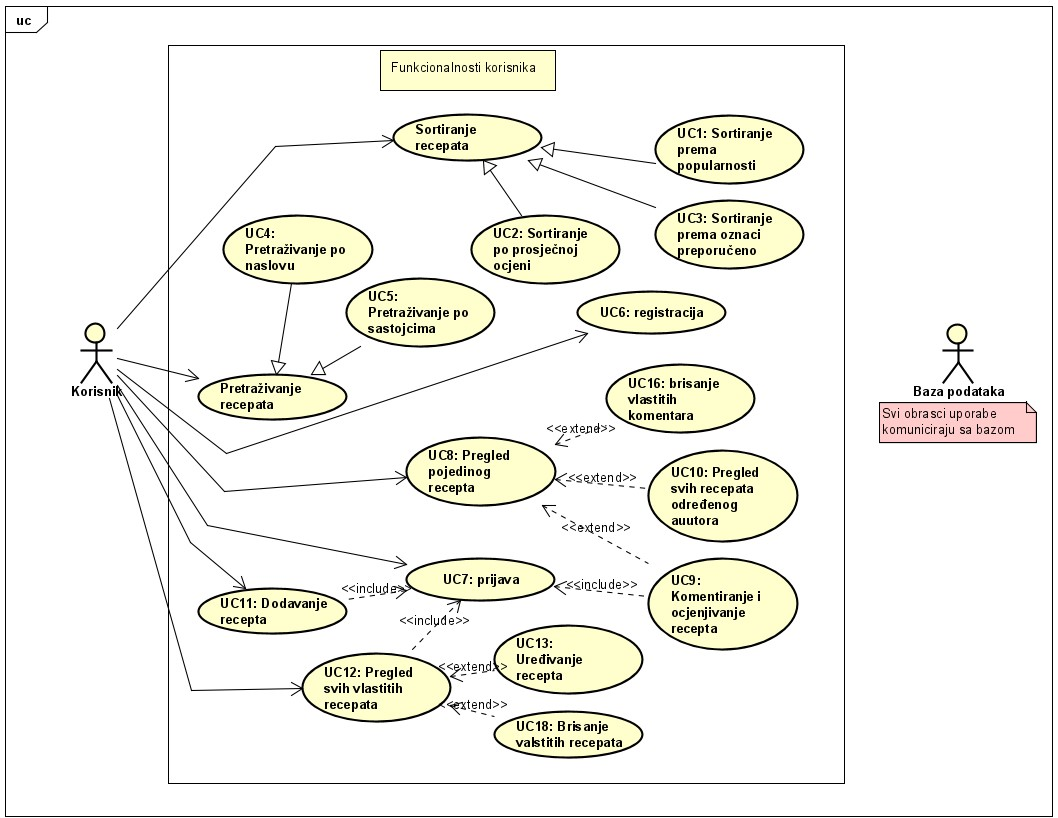
\includegraphics[scale=0.8]{slike/Slika5.jpg} %veličina slike u odnosu na originalnu datoteku i pozicija slike
	\centering
	\caption{Dijagram obrasca uporabe, funkcionalnost korisnika}
	\label{fig:promjene}
\end{figure}

\begin{figure}[H]
	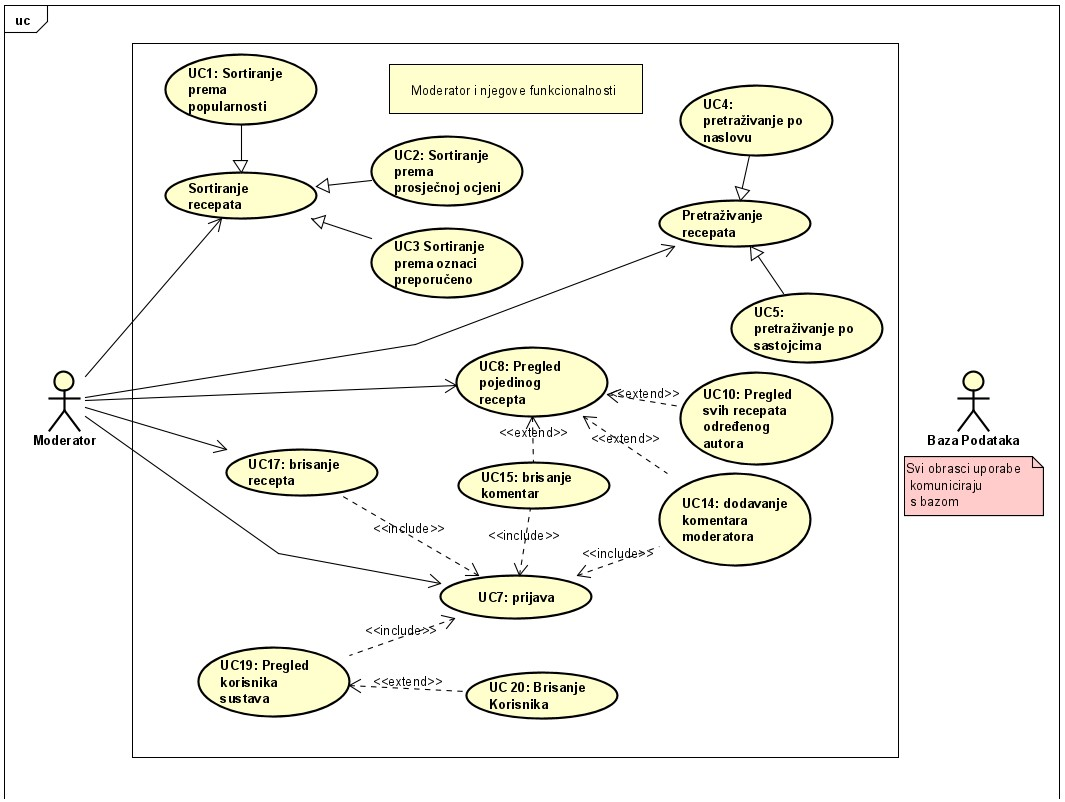
\includegraphics[scale=0.8]{slike/Slika6.jpg} %veličina slike u odnosu na originalnu datoteku i pozicija slike
	\centering
	\caption{Dijagram obrasca uporabe, funkcionalnost moderatora}
	\label{fig:promjene}
\end{figure}

\eject

\subsection{Sekvencijski dijagrami}


\noindent\textbf{Obrazac uporabe UC4 - Pretraživanje recepata po naslovu}\\\\
Klijent na početnoj stranici ima uvid u sve recepte, ali ima i mogućnost filtriranja tih recepata.
Jedno od mogućnosti filtriranja jest filtriranje recepata po naslovu.
Klijent upisuje naslov ili dio naslova kojim želi naći određeni recept te pritišće tipku pretraži.
Pritiskom na tipku, web-apliakcija šalje upit bazi podataka.
Baza podataka pretražuje sve recepte i traži one recepte koji imaju sve riječi ili samo jednu riječ upisanu u tražilicu.
Ukoliko baza podataka ne pronađe niti jedan recept nakon pretraživanja, klijent će biti obaviješten o tome.
U suprotnome, baza podataka vraća web-aplikaciji sve recepte koje je pronašla nakon pretraživanja.
Web-apliakcija potom ispisuje sve recepte klijentu te se time završava pretraživanje.
\begin{figure}[H]
	\includegraphics[scale=0.8]{slike/Slika7.png} %veličina slike u odnosu na originalnu datoteku i pozicija slike
	\centering
	\caption{Sekvencijski dijagram za UC4}
	\label{fig:promjene}
\end{figure}
\pagebreak


\noindent\textbf{Obrazac uporabe UC6 - Registracija}\\\\
Klijent ima mogućnost registracije. Registracija je postupak stvaranja računa po prvi puta u web-aplikaciji.
Klijent pritiskom na gumb "prijava" otvara novu web-stranicu gdje mu je omogućena prijava.
Osim prijave, klijentu je omogućena i registracija, ukoliko nema već postojeći račun.
Klikom na registraciju, pojavljuje se obrazac za stvaranje računa gdje je potrebno unijeti podatke koji će se potom spremati u bazu podataka.
Kako bi obrazac bio uspješno napisan potrebno je: ispuniti sva polja, upisati nepostojeće korisničko ime i lozinku koja se pridržava propisanih pravila.
Ako je klijent uspješno ispunio zahtjev, njegov račun će se spremiti u bazu podataka i dobit će obavijest o uspješnoj registraciji.
Ako klijent nije uspješno ispunio zahtjev, dobit će poruku o odgovarajućoj pogrešci.
\begin{figure}[H]
	\includegraphics[scale=1.0]{slike/Slika8.png} %veličina slike u odnosu na originalnu datoteku i pozicija slike
	\centering
	\caption{Sekvencijski dijagram za UC6}
	\label{fig:promjene}
\end{figure}
\pagebreak

\noindent\textbf{Obrazac uporabe UC11 - Dodavanje recepta}\\\\
Registrirani korisnik (nadalje klijent) ima mogućnost dodavanja recepta.
Dodavanje recepta je vidljivo na profilu klijenta.
Odabirom usluge dodavanja recepta, otvara se web-stranica sa obrascem za dodavanje recepta.
U obrascu je potrebno popuniti označena polja, te priložiti do maksimalno 5 slika.
Ako je klijent uspješno popunio obrazac, recept se dodaje u bazu podataka i klijent dobiva obavijest o uspješnome dodavanju recepta.
Ako klijent nije uspješno popunio obrazac, ispisuje mu se odgovarajuća pogreška, ali se postojeći podaci ne brišu te klijent ima mogućnost ispravljanja pogreške.
\begin{figure}[H]
	\includegraphics[scale=0.8]{slike/Slika9.png} %veličina slike u odnosu na originalnu datoteku i pozicija slike
	\centering
	\caption{Sekvencijski dijagram za UC11}
	\label{fig:promjene}
\end{figure}
\pagebreak

\noindent\textbf{Obrazac uporabe UC13 - Uređivanje recepta}\\\\
Registrirani korisnik (nadalje klijent) ima mogućnost uređivanja vlastitog recepta.
Uređivanje recepta je vidljivo na stranici klijentovog recepta.
Odabirom usluge uređivanja recepta, otvara se web-stranica s već postojećim obrascem.
Podaci u već postojećem obrascu izvučeni su iz baze podataka.
Klijent može dodavati ili brisati podatke u obrascu.
Klijent mora poštovati pravila za uređivanje obrasca kao i kod dodavanja recepta.
Ako je klijent napravio prihvatljivu promjenu, promjena će se spremiti u bazu podataka i klijent dobiva obavijest o uspješnome uređivanju recepta.
Ako je klijent napravio neprihvatljivu promjenu, promjena neće biti spremljena i klijent će dobiti obavijest o pogrešci.
\begin{figure}[H]
	\includegraphics[scale=0.8]{slike/Slika10.png} %veličina slike u odnosu na originalnu datoteku i pozicija slike
	\centering
	\caption{Sekvencijski dijagram za UC13}
	\label{fig:promjene}
\end{figure}
\pagebreak

% \textbf{\textit{dio 1. revizije}}\\

% \textit{Nacrtati sekvencijske dijagrame koji modeliraju najvažnije dijelove sustava (max. 4 dijagrama). Ukoliko postoji nedoumica oko odabira, razjasniti s asistentom. Uz svaki dijagram napisati detaljni opis dijagrama.}
\eject

\section{Ostali zahtjevi}


\textit{
	\begin{packed_item}
		\item Sustav treba omogućiti rad više korisnika u stvarnom vremenu
		\item Korisničko sučelje i sustav moraju podržavati hrvatsku abecedu (dijakritičke
		znakove) pri unosu i prikazu tekstualnog sadržaja
		\item Izvršavanje dijela programa u kojem se pristupa bazi podataka ne smije trajati duže od nekoliko sekundi
		\item Sustav treba biti implementiran kao web aplikacija koristeći objektno-orijentirane jezike
		\item Neispravno korištenje korisničkog sučelja ne smije narušiti funkcionalnost i rad sustava
		\item Sustav treba biti jednostavan za korištenje, korisnici se moraju znati koristiti sučeljem bez opširnih uputa
		\item Nadogradnja sustava ne smije narušavati postojeće funkcionalnosti sustava
		\item Veza s bazom podataka mora biti kvalitetno zaštićena, brza i otporna na vanjske greške
		\item Pristup sustavu mora biti omogućen iz javne mreže pomoću HTTPS.
	\end{packed_item}
}



